\documentclass[a4paper]{scrartcl}
\usepackage[utf8]{inputenc}
\usepackage[english]{babel}
\usepackage{graphicx}
\usepackage{lastpage}
\usepackage{pgf}
\usepackage{wrapfig}
\usepackage{fancyvrb}
\usepackage{fancyhdr}
\pagestyle{fancy}

\usepackage[colorlinks=true,linkcolor=violet]{hyperref}
\usepackage[figure]{hypcap} %jump to img instead of caption text

% Create header and footer
\headheight 27pt
\pagestyle{fancyplain}
\lhead{\footnotesize{Network Programming, ID1212}}
\chead{\footnotesize{Homework 1: Hangman}}
\rhead{}
\lfoot{}
\cfoot{\thepage\ (\pageref{LastPage})}
\rfoot{}

% Create title page
\title{Homework 2: Hangman}
\subtitle{Network Programming, ID1212}
\author{Max Körlinge, korlinge@kth.se}
\date{16 November 2018}

\begin{document}

\maketitle


\section{Introduction}

\noindent The assignment was to develop a distributed application, in this case, a game of Hangman. This assignment builds on a previous assignment and it was requested that this report repeats nothing that was already mentioned in the first report. The requirements for this assignment were:

\begin{itemize}
    \item Communicate using non-blocking TCP sockets.
    \item The nodes must be multithreaded and have a responsive user interface.
    \item The programmed must be designed using a layered architecture and object-oriented design principles.
    \item The program works as expected.
\end{itemize}

There was an optional task to implement a single-threaded event loop architecture in the game server. That task was completed as well.

The program was written in full by the author of this report.

\section{Literature Study}

To prepare for this assignment, all video material provided by the course on non-blocking sockets was viewed together with the code of the sample programs. Important information was gathered on how to communicate with sockets using the Java nio package, and how to use threading for both client and server side programming.

\section{Method}

\noindent Since the previous assignment was completed using layered architecture, the main work was done by substituting the net layers to communicate using non-blocking sockets. To test the ability for the server to handle multiple clients, several clients were started and played with simultaneously while connected to a single server instance. To test that the client's user interface was responsive, the server thread was put to sleep during a request, to see that you could still write commands in the client interface while waiting for a reply. The game was played to see that it still works as expected.

\section{Result}

\noindent The complete source code can be found at \href{https://github.com/fongie/Hangman/tree/nonblocking}{https://github.com/fongie/Hangman/tree/nonblocking}.

\begin{itemize}

	\item To communicate using non-blocking sockets, the Sockets previously used were replaced by Channels and a Selector is created to be able to handle the read, write, and connect operations in a \href{https://github.com/fongie/Hangman/blob/nonblocking/hangmanserver/src/main/java/net/Server.java#L49}{main loop}. New clients are connected on the server by \href{https://github.com/fongie/Hangman/blob/nonblocking/hangmanserver/src/main/java/net/Server.java#L85}{registering} the client channel to the selector and attaching a new \href{https://github.com/fongie/Hangman/blob/nonblocking/hangmanserver/src/main/java/net/Client.java}{Client} object with it. In the previous assignment, the Client objects were run in separate threads, but here they are not, to comply with the requirement on the optional task. The Client object handles the corresponding client channel, that is, prepares to write and receives communication from the player client. On the client side, the process is \href{https://github.com/fongie/Hangman/blob/nonblocking/hangmanclient/src/main/java/net/Connection.java#L84}{similar}, but of course only using a single channel to the server.
	
	\item For a responsive user interface on the client, the user interface is run in one thread while the \href{https://github.com/fongie/Hangman/blob/nonblocking/hangmanclient/src/main/java/net/Connection.java}{Connection} object runs in a separate thread, handling all communication with the server. This means that when communication is being made between client and server, the client still has a responsive user interface.
	
	On the server side, since the Optional task was completed, the clients do not run in multiple threads, but instead they are handled in the single-threaded event loop. This is possible since each new client that connects receive its own selector key with a Client handler object attached to it, and this means that whenever communication is made it can be \href{https://github.com/fongie/Hangman/blob/nonblocking/hangmanserver/src/main/java/net/Server.java#L62}{handled by a particular Client object}, storing the state of the game for that particular user. Because the sockets are non-blocking, threading is not needed to handle multiple clients.
	
	\item The program kept the same design as in the previous assignment, which means that it still complies with object-oriented design principles and layered architecture. One difference worth mentioning is that the \href{https://github.com/fongie/Hangman/blob/nonblocking/hangmanclient/src/main/java/view/UserInterface.java#L56}{Observer} pattern is now employed in the client program to print to the user interface, since some changes had to be made to the threading and using the Consumer interface for the same purpose was no longer applicable.
	
	\item The program works exactly like the previous program, as shown in the requested screenshot (Fig. 1).
	
	\begin{figure}[h!]
  \begin{center}
    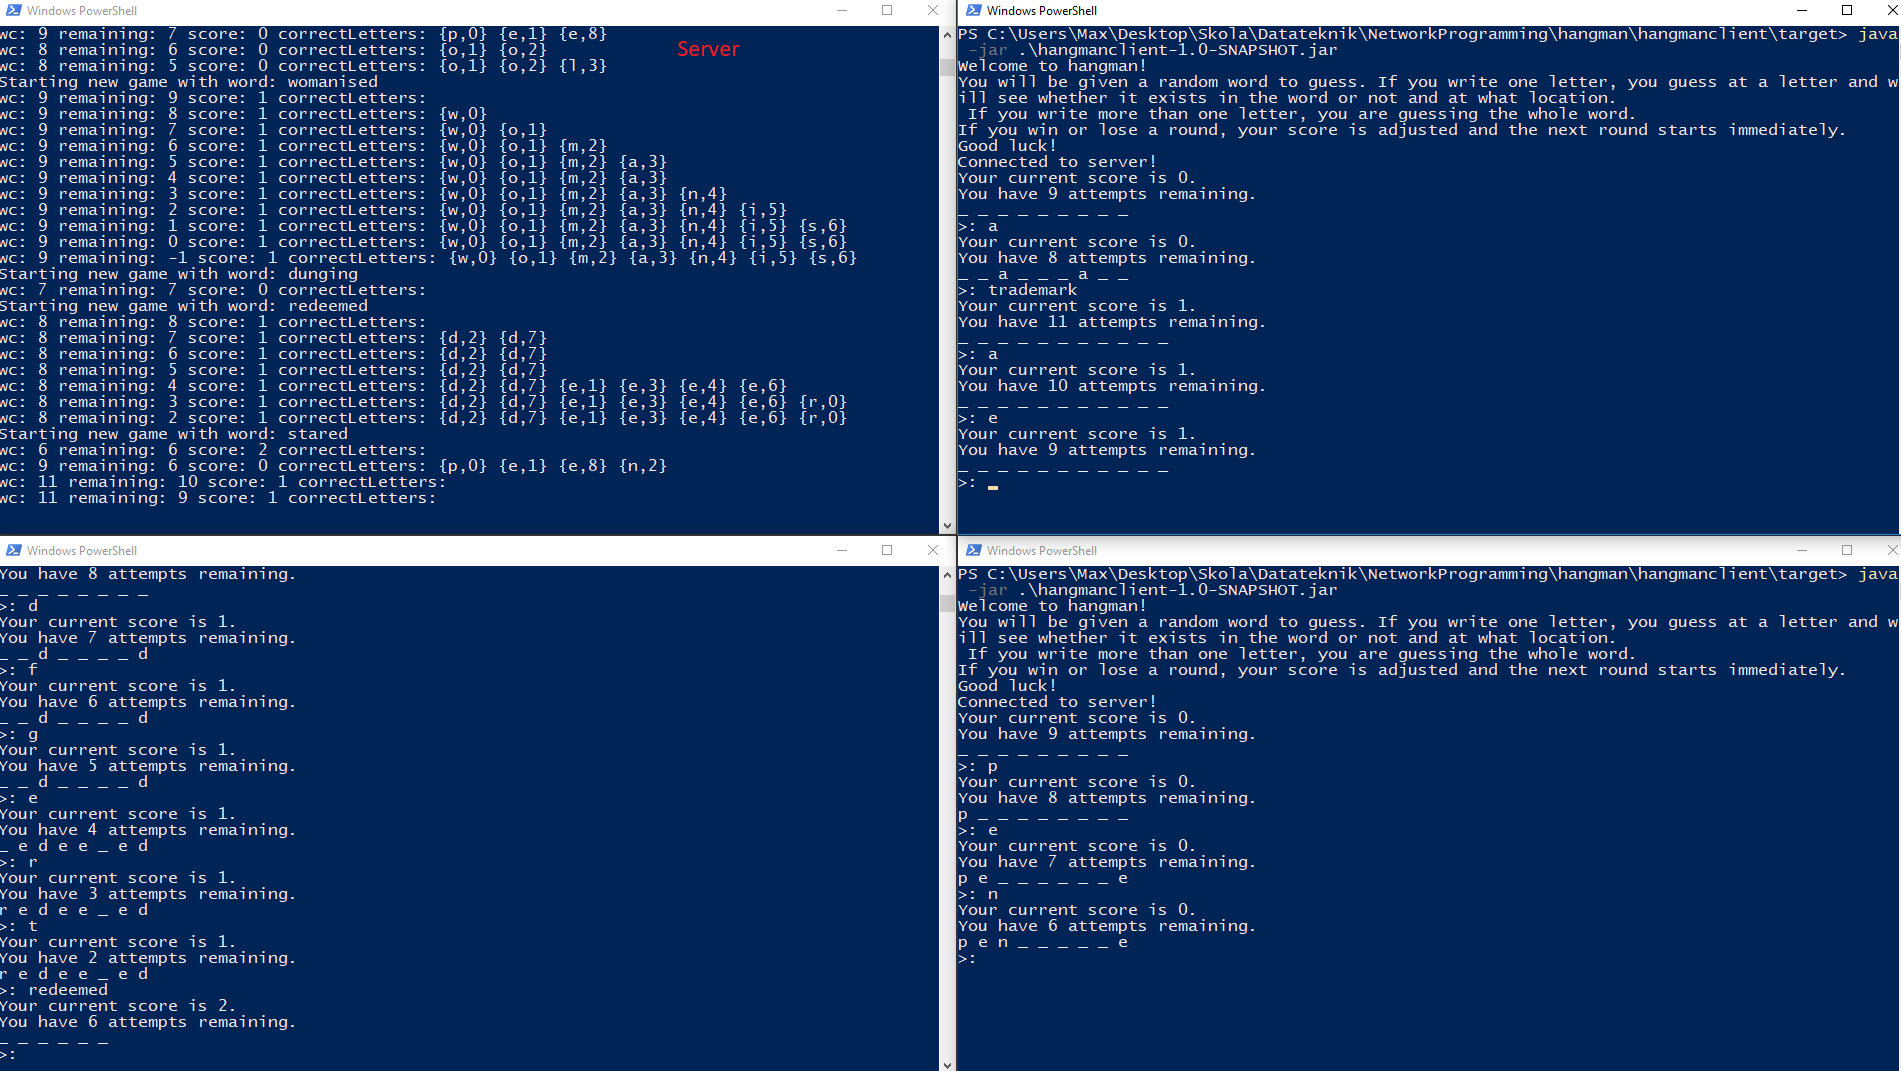
\includegraphics[scale=0.35]{game.png}
    \caption{The server console (top right), and three clients playing simultaneously.}
    \label{fig:game}
  \end{center}
\end{figure}
	
	\item The optional task was, as described above, fulfilled by not running Client handles in their own threads, but using the Selector and its methods to run all clients in a single-threaded event loop. There was an additional part to this task which was to do expensive I/O in a separate thread. This program only has one such operation, namely the picking of the random word from a text file. Since this operation is done at the instantiation of a new Game object, this process is \href{https://github.com/fongie/Hangman/blob/nonblocking/hangmanserver/src/main/java/net/Client.java#L67}{done in a separate thread} as required.
	
\end{itemize}





\section{Discussion}

This assignment was to develop a distributed application using non-blocking sockets, and use threading to achieve a seamless user experience in the client program while being able to entertain several clients in a single thread in the server program. The application was a game of Hangman which was required to have a layered architecture and an informative user interface. As presented above, all the basic and optional requirements were met with.

The main difficulty with this assignment was to get one's head around how the Selector works, and how it can keep track of which channel is which etc. However, once this was clear, it was not very hard to re-use what was created in the last assignment but with new net layers. I had some difficulty finding a reasonable way to use threading with my I/O operation, because the word fetching has to be completed before writing back the new game state to the client, but I think I found a way that works in the end.

I could still improve the user interface given more time, as mentioned in the last report, but that was outside of the requirements of this assignment as well.

\section{Comments About the Course}

I spent about 8 hours on the lecture material, about 8 hours on the assignment, and about 2 hours to write the report, making 18 hours in total.

\end{document}
